%!TEX root = ../../controlbook.tex

\chapter{Design Study: Mass Spring Damper}
\label{hw:mass}

%\addcontentsline{toc}{chapter}{\hspace{1cm} Design Study D: Mass Spring Damper}

\begin{wrapfigure}{r}{0.6\textwidth}
  % Requires \usepackage{graphicx}
  \centering
  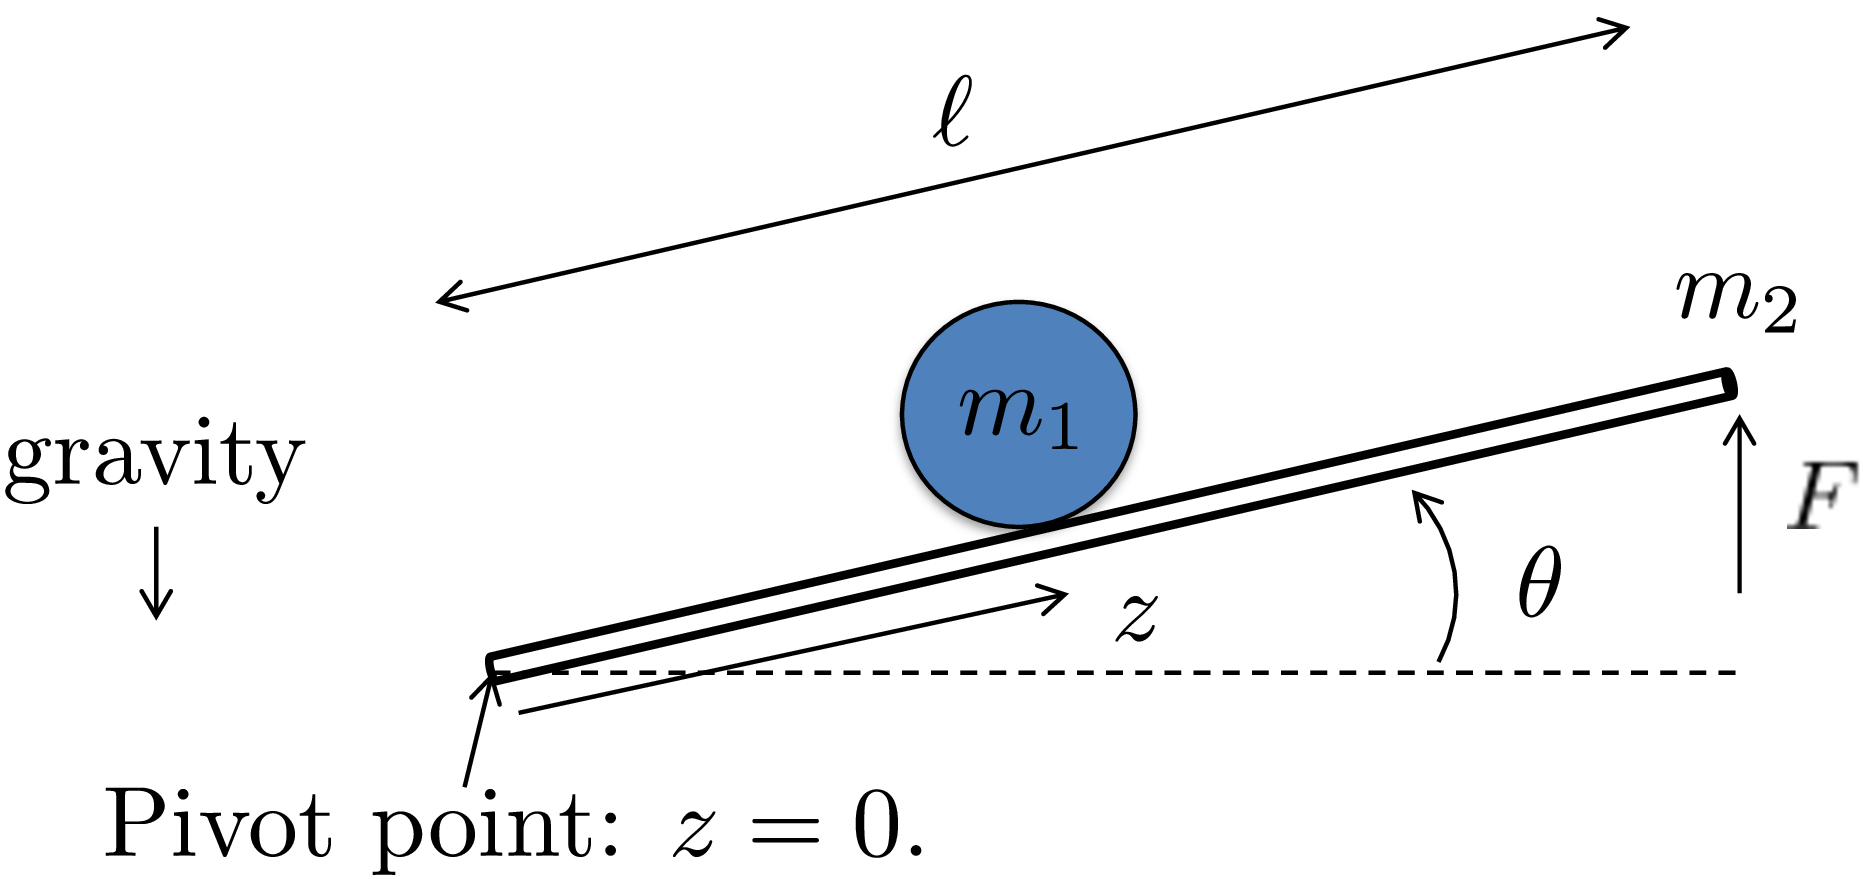
\includegraphics[width=0.59\textwidth]{6_design_studies/figures/hw_ballbeam_defn}\\
  \caption{Ball on Beam Problem}
  \label{fig:ballbeam_defn}
\end{wrapfigure}

%\controlbookfigure{0.5}
%	{6_design_studies/figures/hw_ballbeam_defn}
%	{Ball on Beam.}
%	{fig:ballbeam_defn}

Figure~\ref{fig:ballbeam_defn} shows the \index{ball and beam} system.  The position of the ball measured from the pivot point is $z$ and the speed of the ball along the direction of the beam is $\dot{z}$.  The angle of the beam from level is $\theta$ and the angular speed of the beam is $\dot{\theta}$.  Gravity acts in the down direction.  The mass of the ball is $m_1$ and the mass of the beam is $m_2$.  The length of the beam is $\ell$.  An external force is applied at the end of the beam as shown in \fref{fig:ballbeam_defn}.  

Use the following physical parameters: $m_1=0.35$~kg, $m_2=2$~kg, $\ell=0.5$~m, $g=9.8$~m/s$^2$.



\vspace{.5cm}

%!TEX root = ../../controlbook.tex

%\begin{table}[ht!]
%\fcolorbox{realred}{none}%
%{\begin{minipage}{8.31cm}%
	

\par\noindent{\bf Examples (with solutions):}
\begin{multicols}{2}
\begin{description}
\setlength{\itemsep}{0pt}
\setlength{\parskip}{0pt}
	\item {\bf\controlbookhyperref{hw:arm_kinetic}{ A.2}} Kinetic energy.
%	\item {\bf\controlbookhyperref{hw:arm_kinetic}{ A.2}} Animation for simuation.	
	\item {\bf\controlbookhyperref{hw:arm_equations_of_motion}{ A.3}} Equations of motion.
%	\item {\bf\controlbookhyperref{hw:arm_equations_of_motion}{ A.3}} Simulate equations of motion.
	\item {\bf\controlbookhyperref{hw:arm_linearization}{ A.4}} Linearize equations of motion.
	\item {\bf\controlbookhyperref{hw:arm_transfer_function}{ A.5}} Transfer function model.
	\item {\bf\controlbookhyperref{hw:arm_state_space}{ A.6}} State space model.
	\item {\bf\controlbookhyperref{hw:arm_pd_pole_placement}{ A.7}} Pole placement using PD.
	\item {\bf\controlbookhyperref{hw:arm_PD_design}{ A.8}} Second order design.
	\item {\bf\controlbookhyperref{hw:arm_system_type}{ A.9}} Integrators and system type.
	\item {\bf\controlbookhyperref{hw:arm_root_locus}{A.P.6}} Root locus.
	\item {\bf\controlbookhyperref{hw:arm_digital_PID}{ A.10}} Digital PID.
	\item {\bf\controlbookhyperref{hw:arm_state_feedback}{ A.11}} Full state feedback.
	\item {\bf\controlbookhyperref{hw:arm_integrator_state_feedback}{ A.12}} Full state with integrator.
	\item {\bf\controlbookhyperref{hw:arm_observer}{ A.13}} Observer based control.
	\item {\bf\controlbookhyperref{hw:arm_disturbance_observer}{ A.14}} Disturbance observer.
	\item {\bf\controlbookhyperref{hw:arm_bode}{ A.15}} Frequency Response.
	\item {\bf\controlbookhyperref{hw:arm_loopgain}{ A.16}} Loop gain.
	\item {\bf\controlbookhyperref{hw:arm_margins}{ A.17}} Stability margins.
	\item {\bf\controlbookhyperref{hw:arm_loopshaping}{ A.18}} Loopshaping design.
\end{description}
\end{multicols}

Note: The notation identifies the design configuration and the chapter
in which it is used: {\bf Example A.4} refers to the application of
approximations in Chapter~4 to linearize design
configuration~A\@. Similarly, {\bf Example A.P.6} refers to the root locus assignment 
associated with Appendix A.P.6.

%\end{minipage}}
%\end{table}

\clearpage

	\section*{
		\controlbookhyperref{hw:mass}
			{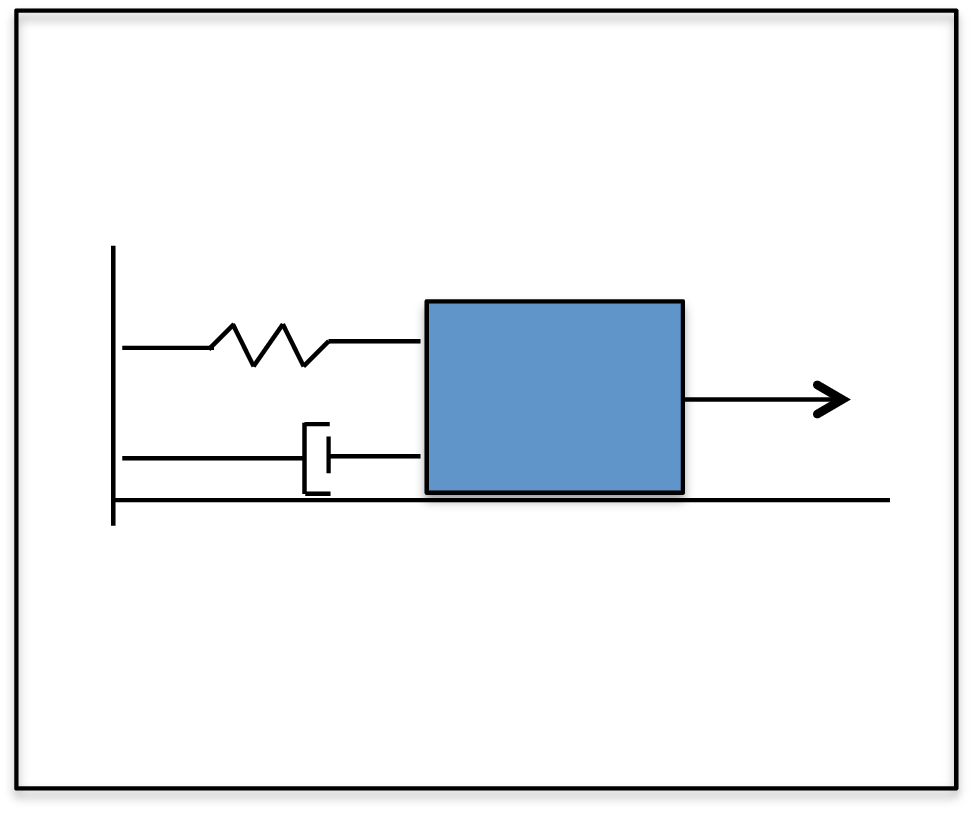
\includegraphics[width=0.1\textwidth]{6_design_studies/figures/hw_mass_thumbnail.pdf}}
		Homework \ref{hw:mass}.\ref{chap:kinetic-energy}} \label{hw:mass_kinetic}
		\begin{description} \item[]
\item[(a)] Modify the state feedback solution developed in Homework~\ref{hw:vtol}.\ref{chap:state-feedback} to add an integrator with anti-windup to the altitude feedback loop and to the position feedback loop.
\item[(b)] Allow the plant parameters to vary up to 20\% and add a constant input disturbance of $0.1$~Newtons to the input of position dynamics simulating wind.  {\it Hint:  The best place to add the wind force is in the class that implements the dynamics.  For example, one possibility is to modify the $z$ dynamics as 

\texttt{zddot = (-(fr+fl)*sin(theta)+F\_wind)/(P.mc+2*P.mr)}.}

\item[(c)] Tune the integrator poles on both loops (and other gains if necessary) to get good tracking performance.  
\end{description}


%		\subsection*{Solution}
Python code used to design the observer based controller is shown below:
%\iftoggle{soln}{%
%  \lstinputlisting{simulink_e13/param.m}
%}{%
%  \lstinputlisting{./6_design_studies/_E_ballbeam/simulink/hw13/ballbeamParamHW13.m}
%}
\ifsolutionmanual
\lstinputlisting{./6_design_studies/_e_ballbeam/python/hw13/ballbeamParamHW13.py}
\else
\lstinputlisting{../../python/hw13/ballbeamParamHW13.py}
\fi


Python code for the observer based control  is shown below:
%\iftoggle{soln}{%
%  \lstinputlisting{simulink_e13/ballbeam_ctrl.m}
%}{%
%  \lstinputlisting{./6_design_studies/_E_ballbeam/simulink/hw13/ballbeam_ctrl.m}
%}
\ifsolutionmanual
\lstinputlisting{./6_design_studies/_e_ballbeam/python/hw13/ballBeamController.py}
\else
\lstinputlisting{../../python/hw13/ballBeamController.py}
\fi


See the wiki for the complete solution.


%	\section*{
%		\controlbookhyperref{hw:mass}{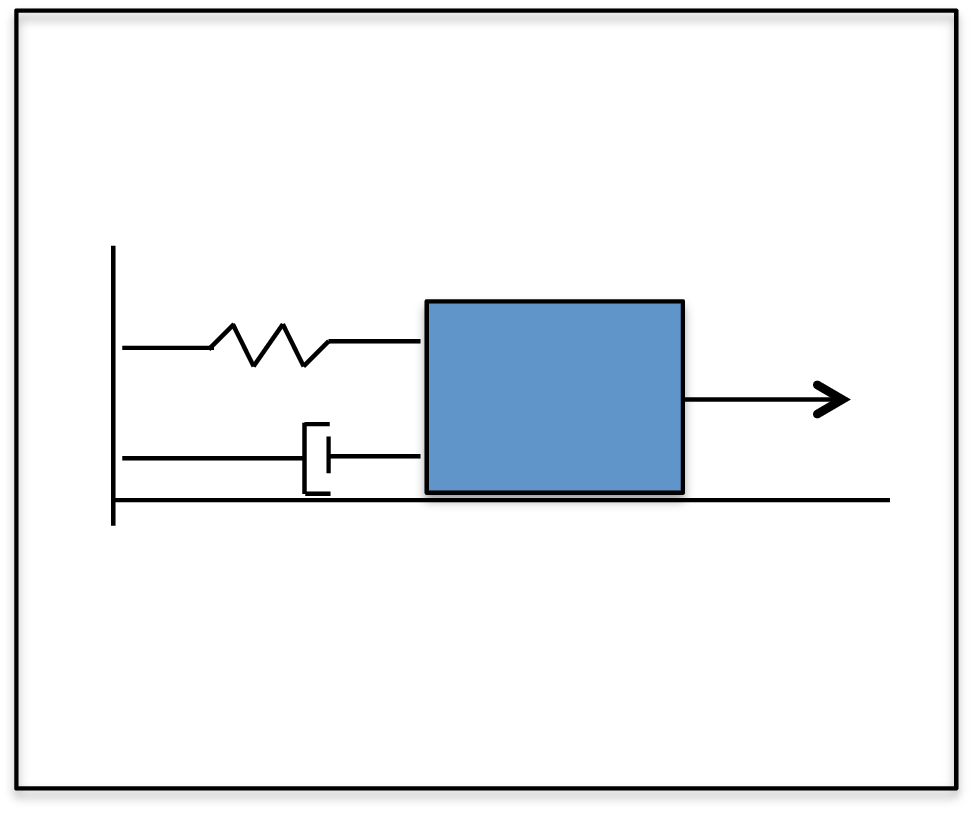
\includegraphics[width=0.1\textwidth]{6_design_studies/figures/hw_mass_thumbnail.pdf}}
%		Homework \ref{hw:mass}.\ref{chap:animation}}  \label{hw:mass_animation}
%		\begin{description} \item[]
\item[(a)] Modify the state feedback solution developed in Homework~\ref{hw:vtol}.\ref{chap:state-feedback} to add an integrator with anti-windup to the altitude feedback loop and to the position feedback loop.
\item[(b)] Allow the plant parameters to vary up to 20\% and add a constant input disturbance of $0.1$~Newtons to the input of position dynamics simulating wind.  {\it Hint:  The best place to add the wind force is in the class that implements the dynamics.  For example, one possibility is to modify the $z$ dynamics as 

\texttt{zddot = (-(fr+fl)*sin(theta)+F\_wind)/(P.mc+2*P.mr)}.}

\item[(c)] Tune the integrator poles on both loops (and other gains if necessary) to get good tracking performance.  
\end{description}

%%		\subsection*{Solution}
Python code used to design the observer based controller is shown below:
%\iftoggle{soln}{%
%  \lstinputlisting{simulink_e13/param.m}
%}{%
%  \lstinputlisting{./6_design_studies/_E_ballbeam/simulink/hw13/ballbeamParamHW13.m}
%}
\ifsolutionmanual
\lstinputlisting{./6_design_studies/_e_ballbeam/python/hw13/ballbeamParamHW13.py}
\else
\lstinputlisting{../../python/hw13/ballbeamParamHW13.py}
\fi


Python code for the observer based control  is shown below:
%\iftoggle{soln}{%
%  \lstinputlisting{simulink_e13/ballbeam_ctrl.m}
%}{%
%  \lstinputlisting{./6_design_studies/_E_ballbeam/simulink/hw13/ballbeam_ctrl.m}
%}
\ifsolutionmanual
\lstinputlisting{./6_design_studies/_e_ballbeam/python/hw13/ballBeamController.py}
\else
\lstinputlisting{../../python/hw13/ballBeamController.py}
\fi


See the wiki for the complete solution.


	\section*{
		\controlbookhyperref{hw:mass}{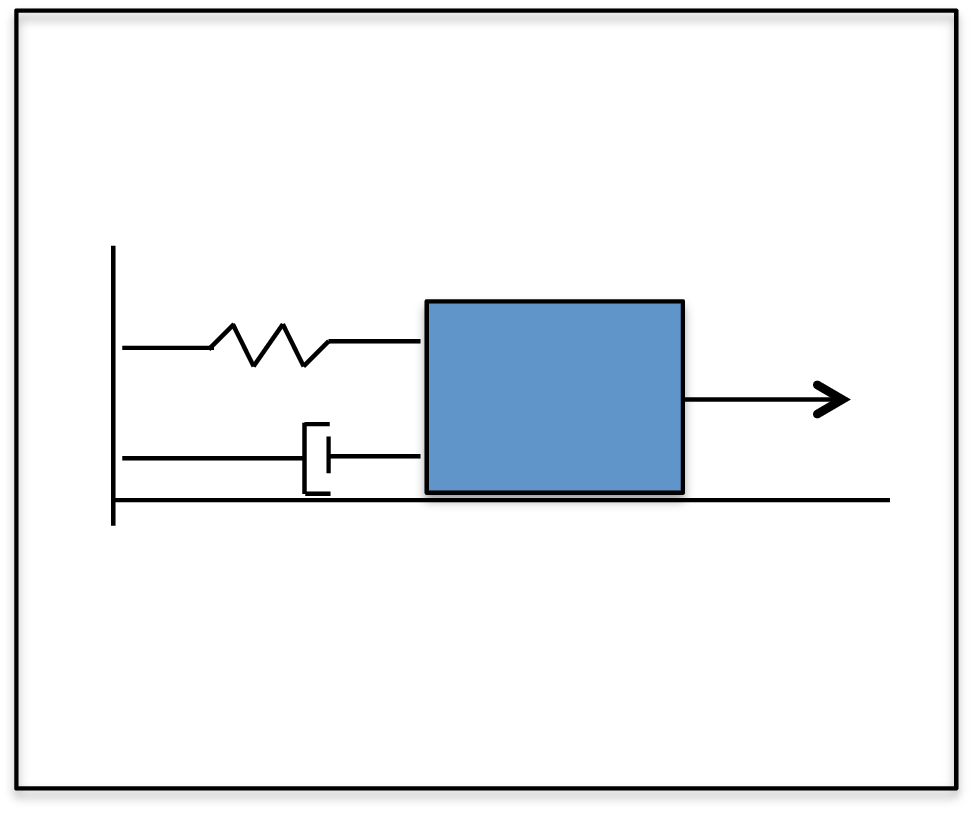
\includegraphics[width=0.1\textwidth]{6_design_studies/figures/hw_mass_thumbnail.pdf}}
		Homework \ref{hw:mass}.\ref{chap:euler-lagrange}}  		
		\label{hw:mass_equations_of_motion}
		\begin{description} \item[]
\item[(a)] Modify the state feedback solution developed in Homework~\ref{hw:vtol}.\ref{chap:state-feedback} to add an integrator with anti-windup to the altitude feedback loop and to the position feedback loop.
\item[(b)] Allow the plant parameters to vary up to 20\% and add a constant input disturbance of $0.1$~Newtons to the input of position dynamics simulating wind.  {\it Hint:  The best place to add the wind force is in the class that implements the dynamics.  For example, one possibility is to modify the $z$ dynamics as 

\texttt{zddot = (-(fr+fl)*sin(theta)+F\_wind)/(P.mc+2*P.mr)}.}

\item[(c)] Tune the integrator poles on both loops (and other gains if necessary) to get good tracking performance.  
\end{description}


%		\subsection*{Solution}
Python code used to design the observer based controller is shown below:
%\iftoggle{soln}{%
%  \lstinputlisting{simulink_e13/param.m}
%}{%
%  \lstinputlisting{./6_design_studies/_E_ballbeam/simulink/hw13/ballbeamParamHW13.m}
%}
\ifsolutionmanual
\lstinputlisting{./6_design_studies/_e_ballbeam/python/hw13/ballbeamParamHW13.py}
\else
\lstinputlisting{../../python/hw13/ballbeamParamHW13.py}
\fi


Python code for the observer based control  is shown below:
%\iftoggle{soln}{%
%  \lstinputlisting{simulink_e13/ballbeam_ctrl.m}
%}{%
%  \lstinputlisting{./6_design_studies/_E_ballbeam/simulink/hw13/ballbeam_ctrl.m}
%}
\ifsolutionmanual
\lstinputlisting{./6_design_studies/_e_ballbeam/python/hw13/ballBeamController.py}
\else
\lstinputlisting{../../python/hw13/ballBeamController.py}
\fi


See the wiki for the complete solution.


%	\section*{
%		\controlbookhyperref{hw:mass}{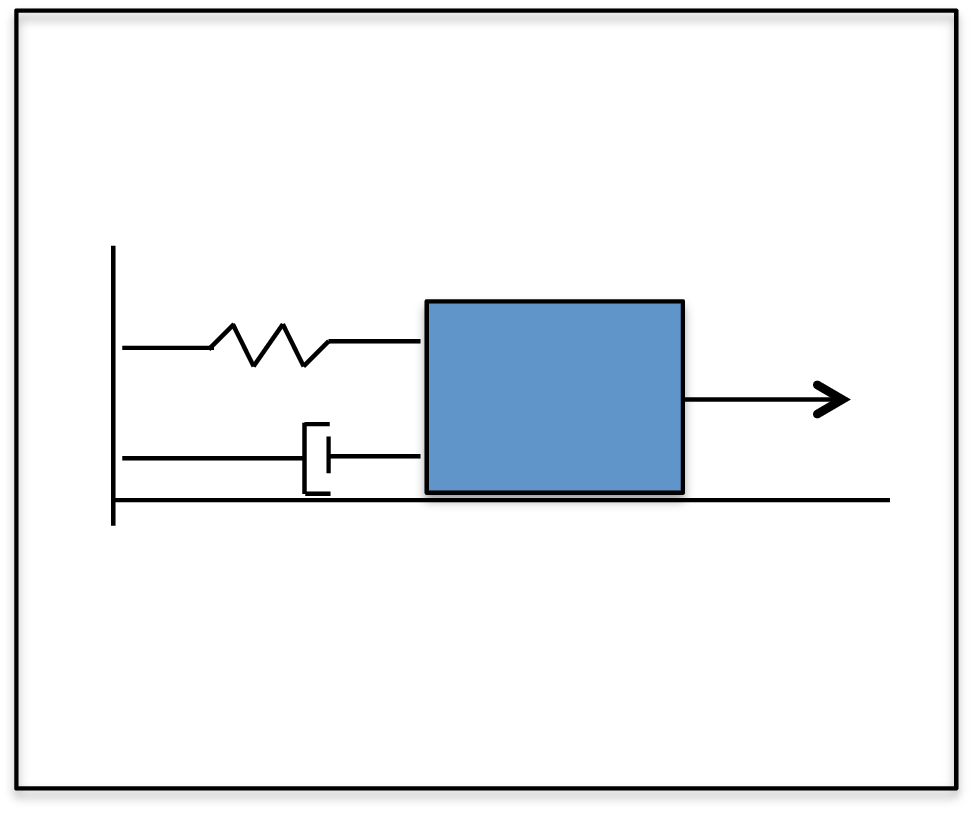
\includegraphics[width=0.1\textwidth]{6_design_studies/figures/hw_mass_thumbnail.pdf}}
%		Homework \ref{hw:mass}.\ref{chap:s_functions}}  \label{hw:mass_s_function}
%		\begin{description} \item[]
\item[(a)] Modify the state feedback solution developed in Homework~\ref{hw:vtol}.\ref{chap:state-feedback} to add an integrator with anti-windup to the altitude feedback loop and to the position feedback loop.
\item[(b)] Allow the plant parameters to vary up to 20\% and add a constant input disturbance of $0.1$~Newtons to the input of position dynamics simulating wind.  {\it Hint:  The best place to add the wind force is in the class that implements the dynamics.  For example, one possibility is to modify the $z$ dynamics as 

\texttt{zddot = (-(fr+fl)*sin(theta)+F\_wind)/(P.mc+2*P.mr)}.}

\item[(c)] Tune the integrator poles on both loops (and other gains if necessary) to get good tracking performance.  
\end{description}

	\section*{
		\controlbookhyperref{hw:mass}{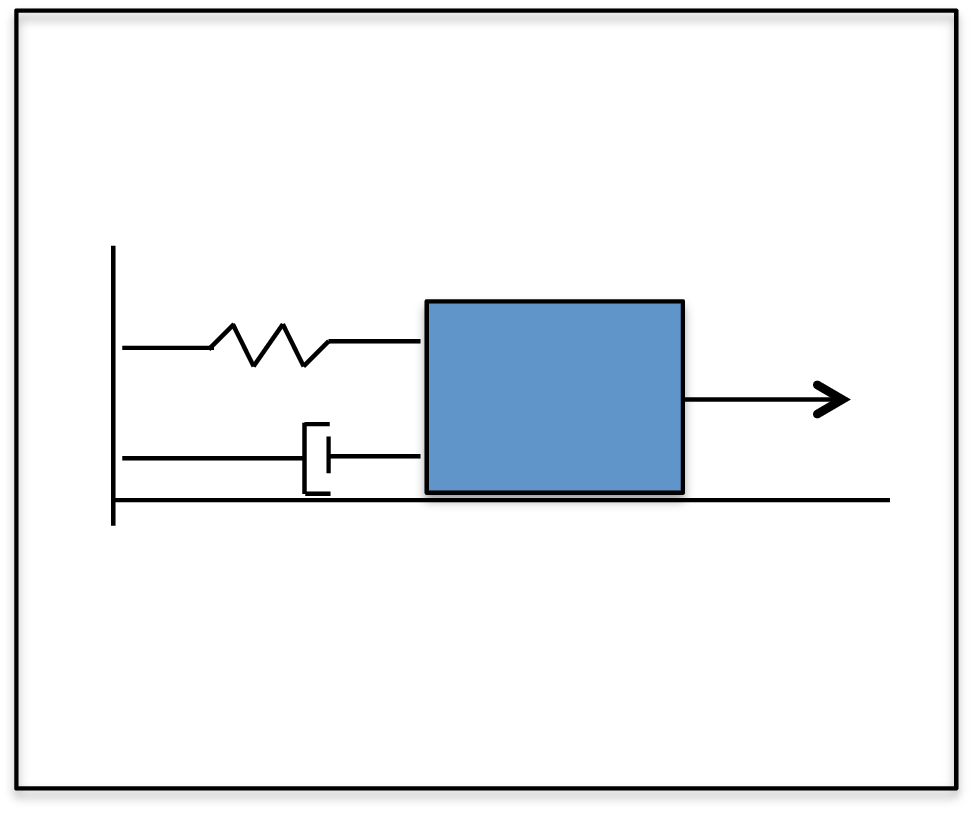
\includegraphics[width=0.1\textwidth]{6_design_studies/figures/hw_mass_thumbnail.pdf}}
		Homework \ref{hw:mass}.\ref{chap:linearization}}  \label{hw:mass_linearization}
		\begin{description} \item[]
\item[(a)] Modify the state feedback solution developed in Homework~\ref{hw:vtol}.\ref{chap:state-feedback} to add an integrator with anti-windup to the altitude feedback loop and to the position feedback loop.
\item[(b)] Allow the plant parameters to vary up to 20\% and add a constant input disturbance of $0.1$~Newtons to the input of position dynamics simulating wind.  {\it Hint:  The best place to add the wind force is in the class that implements the dynamics.  For example, one possibility is to modify the $z$ dynamics as 

\texttt{zddot = (-(fr+fl)*sin(theta)+F\_wind)/(P.mc+2*P.mr)}.}

\item[(c)] Tune the integrator poles on both loops (and other gains if necessary) to get good tracking performance.  
\end{description}

%		\subsection*{Solution}
Python code used to design the observer based controller is shown below:
%\iftoggle{soln}{%
%  \lstinputlisting{simulink_e13/param.m}
%}{%
%  \lstinputlisting{./6_design_studies/_E_ballbeam/simulink/hw13/ballbeamParamHW13.m}
%}
\ifsolutionmanual
\lstinputlisting{./6_design_studies/_e_ballbeam/python/hw13/ballbeamParamHW13.py}
\else
\lstinputlisting{../../python/hw13/ballbeamParamHW13.py}
\fi


Python code for the observer based control  is shown below:
%\iftoggle{soln}{%
%  \lstinputlisting{simulink_e13/ballbeam_ctrl.m}
%}{%
%  \lstinputlisting{./6_design_studies/_E_ballbeam/simulink/hw13/ballbeam_ctrl.m}
%}
\ifsolutionmanual
\lstinputlisting{./6_design_studies/_e_ballbeam/python/hw13/ballBeamController.py}
\else
\lstinputlisting{../../python/hw13/ballBeamController.py}
\fi


See the wiki for the complete solution.


	\section*{
		\controlbookhyperref{hw:mass}{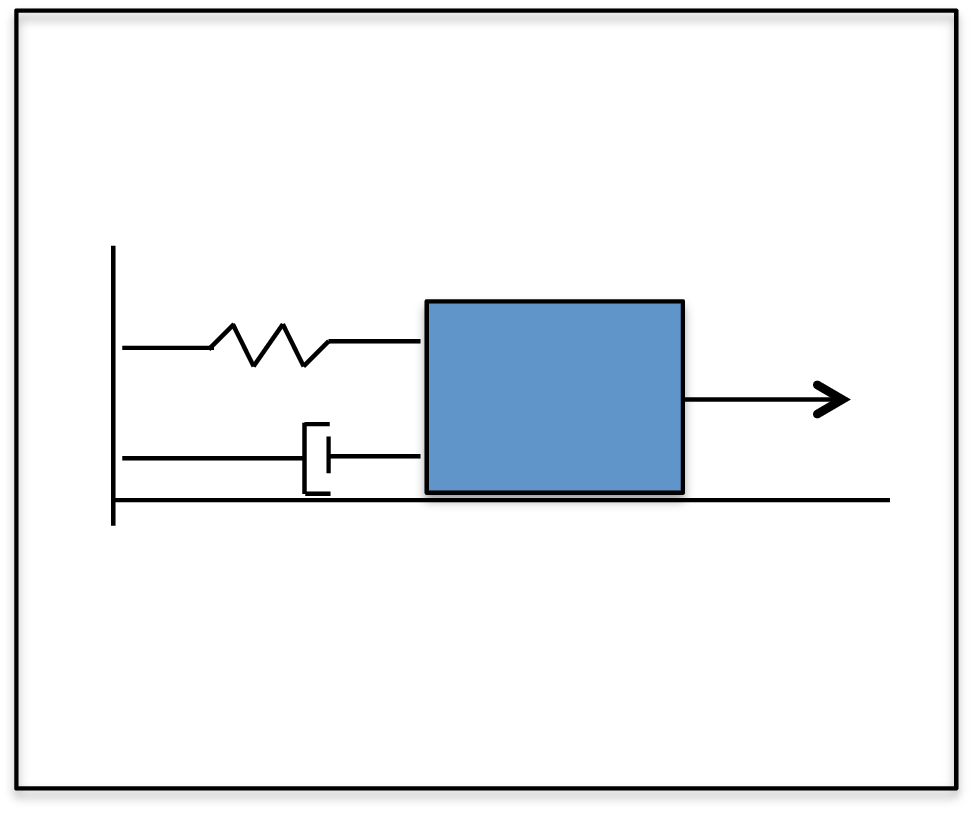
\includegraphics[width=0.1\textwidth]{6_design_studies/figures/hw_mass_thumbnail.pdf}}
		Homework \ref{hw:mass}.\ref{chap:transfer_function_models}}  \label{hw:mass_transfer_function}
		\begin{description} \item[]
\item[(a)] Modify the state feedback solution developed in Homework~\ref{hw:vtol}.\ref{chap:state-feedback} to add an integrator with anti-windup to the altitude feedback loop and to the position feedback loop.
\item[(b)] Allow the plant parameters to vary up to 20\% and add a constant input disturbance of $0.1$~Newtons to the input of position dynamics simulating wind.  {\it Hint:  The best place to add the wind force is in the class that implements the dynamics.  For example, one possibility is to modify the $z$ dynamics as 

\texttt{zddot = (-(fr+fl)*sin(theta)+F\_wind)/(P.mc+2*P.mr)}.}

\item[(c)] Tune the integrator poles on both loops (and other gains if necessary) to get good tracking performance.  
\end{description}

%		\subsection*{Solution}
Python code used to design the observer based controller is shown below:
%\iftoggle{soln}{%
%  \lstinputlisting{simulink_e13/param.m}
%}{%
%  \lstinputlisting{./6_design_studies/_E_ballbeam/simulink/hw13/ballbeamParamHW13.m}
%}
\ifsolutionmanual
\lstinputlisting{./6_design_studies/_e_ballbeam/python/hw13/ballbeamParamHW13.py}
\else
\lstinputlisting{../../python/hw13/ballbeamParamHW13.py}
\fi


Python code for the observer based control  is shown below:
%\iftoggle{soln}{%
%  \lstinputlisting{simulink_e13/ballbeam_ctrl.m}
%}{%
%  \lstinputlisting{./6_design_studies/_E_ballbeam/simulink/hw13/ballbeam_ctrl.m}
%}
\ifsolutionmanual
\lstinputlisting{./6_design_studies/_e_ballbeam/python/hw13/ballBeamController.py}
\else
\lstinputlisting{../../python/hw13/ballBeamController.py}
\fi


See the wiki for the complete solution.


	\section*{
		\controlbookhyperref{hw:mass}{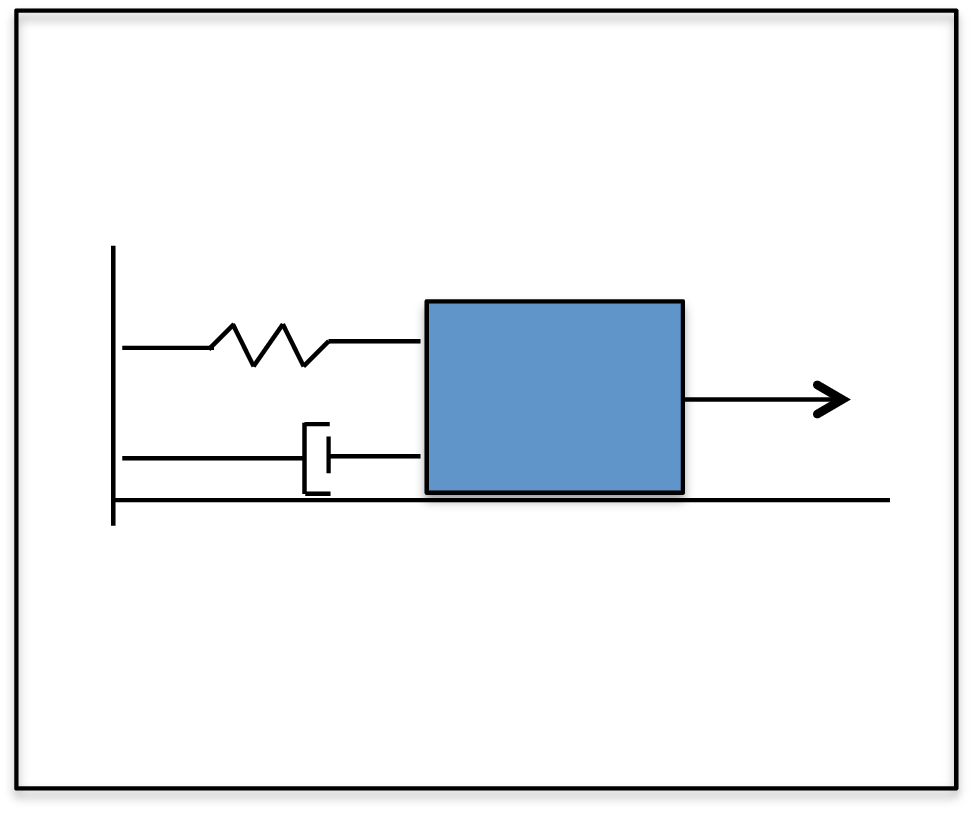
\includegraphics[width=0.1\textwidth]{6_design_studies/figures/hw_mass_thumbnail.pdf}}
		Homework \ref{hw:mass}.\ref{chap:state_space_models}}  \label{hw:mass_state_space}
		\begin{description} \item[]
\item[(a)] Modify the state feedback solution developed in Homework~\ref{hw:vtol}.\ref{chap:state-feedback} to add an integrator with anti-windup to the altitude feedback loop and to the position feedback loop.
\item[(b)] Allow the plant parameters to vary up to 20\% and add a constant input disturbance of $0.1$~Newtons to the input of position dynamics simulating wind.  {\it Hint:  The best place to add the wind force is in the class that implements the dynamics.  For example, one possibility is to modify the $z$ dynamics as 

\texttt{zddot = (-(fr+fl)*sin(theta)+F\_wind)/(P.mc+2*P.mr)}.}

\item[(c)] Tune the integrator poles on both loops (and other gains if necessary) to get good tracking performance.  
\end{description}

%		\subsection*{Solution}
Python code used to design the observer based controller is shown below:
%\iftoggle{soln}{%
%  \lstinputlisting{simulink_e13/param.m}
%}{%
%  \lstinputlisting{./6_design_studies/_E_ballbeam/simulink/hw13/ballbeamParamHW13.m}
%}
\ifsolutionmanual
\lstinputlisting{./6_design_studies/_e_ballbeam/python/hw13/ballbeamParamHW13.py}
\else
\lstinputlisting{../../python/hw13/ballbeamParamHW13.py}
\fi


Python code for the observer based control  is shown below:
%\iftoggle{soln}{%
%  \lstinputlisting{simulink_e13/ballbeam_ctrl.m}
%}{%
%  \lstinputlisting{./6_design_studies/_E_ballbeam/simulink/hw13/ballbeam_ctrl.m}
%}
\ifsolutionmanual
\lstinputlisting{./6_design_studies/_e_ballbeam/python/hw13/ballBeamController.py}
\else
\lstinputlisting{../../python/hw13/ballBeamController.py}
\fi


See the wiki for the complete solution.


	\section*{
		\controlbookhyperref{hw:mass}{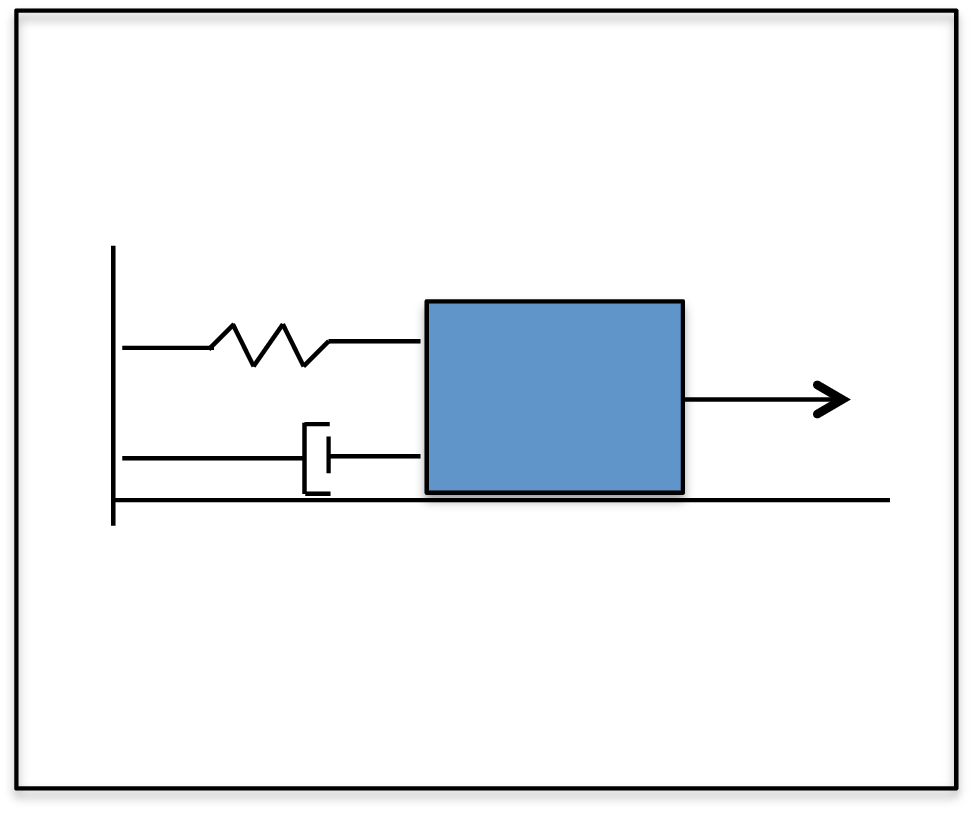
\includegraphics[width=0.1\textwidth]{6_design_studies/figures/hw_mass_thumbnail.pdf}}
		Homework \ref{hw:mass}.\ref{chap:PID-pole-placement}}  \label{hw:mass_pd_pole_placement}
		\begin{description} \item[]
\item[(a)] Modify the state feedback solution developed in Homework~\ref{hw:vtol}.\ref{chap:state-feedback} to add an integrator with anti-windup to the altitude feedback loop and to the position feedback loop.
\item[(b)] Allow the plant parameters to vary up to 20\% and add a constant input disturbance of $0.1$~Newtons to the input of position dynamics simulating wind.  {\it Hint:  The best place to add the wind force is in the class that implements the dynamics.  For example, one possibility is to modify the $z$ dynamics as 

\texttt{zddot = (-(fr+fl)*sin(theta)+F\_wind)/(P.mc+2*P.mr)}.}

\item[(c)] Tune the integrator poles on both loops (and other gains if necessary) to get good tracking performance.  
\end{description}

%		\subsection*{Solution}
Python code used to design the observer based controller is shown below:
%\iftoggle{soln}{%
%  \lstinputlisting{simulink_e13/param.m}
%}{%
%  \lstinputlisting{./6_design_studies/_E_ballbeam/simulink/hw13/ballbeamParamHW13.m}
%}
\ifsolutionmanual
\lstinputlisting{./6_design_studies/_e_ballbeam/python/hw13/ballbeamParamHW13.py}
\else
\lstinputlisting{../../python/hw13/ballbeamParamHW13.py}
\fi


Python code for the observer based control  is shown below:
%\iftoggle{soln}{%
%  \lstinputlisting{simulink_e13/ballbeam_ctrl.m}
%}{%
%  \lstinputlisting{./6_design_studies/_E_ballbeam/simulink/hw13/ballbeam_ctrl.m}
%}
\ifsolutionmanual
\lstinputlisting{./6_design_studies/_e_ballbeam/python/hw13/ballBeamController.py}
\else
\lstinputlisting{../../python/hw13/ballBeamController.py}
\fi


See the wiki for the complete solution.


	\section*{
		\controlbookhyperref{hw:mass}{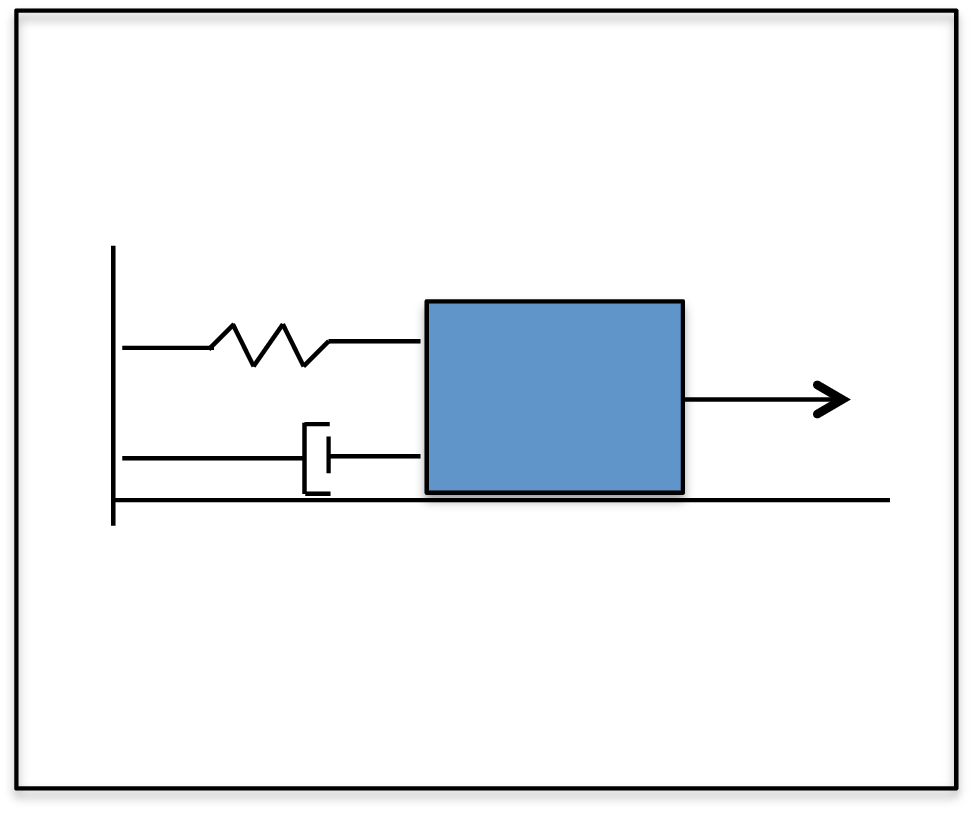
\includegraphics[width=0.1\textwidth]{6_design_studies/figures/hw_mass_thumbnail.pdf}}
		Homework \ref{hw:mass}.\ref{chap:PID-design-specs}}  \label{hw:mass_time_spec}
		\begin{description} \item[]
\item[(a)] Modify the state feedback solution developed in Homework~\ref{hw:vtol}.\ref{chap:state-feedback} to add an integrator with anti-windup to the altitude feedback loop and to the position feedback loop.
\item[(b)] Allow the plant parameters to vary up to 20\% and add a constant input disturbance of $0.1$~Newtons to the input of position dynamics simulating wind.  {\it Hint:  The best place to add the wind force is in the class that implements the dynamics.  For example, one possibility is to modify the $z$ dynamics as 

\texttt{zddot = (-(fr+fl)*sin(theta)+F\_wind)/(P.mc+2*P.mr)}.}

\item[(c)] Tune the integrator poles on both loops (and other gains if necessary) to get good tracking performance.  
\end{description}

%		\subsection*{Solution}
Python code used to design the observer based controller is shown below:
%\iftoggle{soln}{%
%  \lstinputlisting{simulink_e13/param.m}
%}{%
%  \lstinputlisting{./6_design_studies/_E_ballbeam/simulink/hw13/ballbeamParamHW13.m}
%}
\ifsolutionmanual
\lstinputlisting{./6_design_studies/_e_ballbeam/python/hw13/ballbeamParamHW13.py}
\else
\lstinputlisting{../../python/hw13/ballbeamParamHW13.py}
\fi


Python code for the observer based control  is shown below:
%\iftoggle{soln}{%
%  \lstinputlisting{simulink_e13/ballbeam_ctrl.m}
%}{%
%  \lstinputlisting{./6_design_studies/_E_ballbeam/simulink/hw13/ballbeam_ctrl.m}
%}
\ifsolutionmanual
\lstinputlisting{./6_design_studies/_e_ballbeam/python/hw13/ballBeamController.py}
\else
\lstinputlisting{../../python/hw13/ballBeamController.py}
\fi


See the wiki for the complete solution.


	\section*{
		\controlbookhyperref{hw:mass}{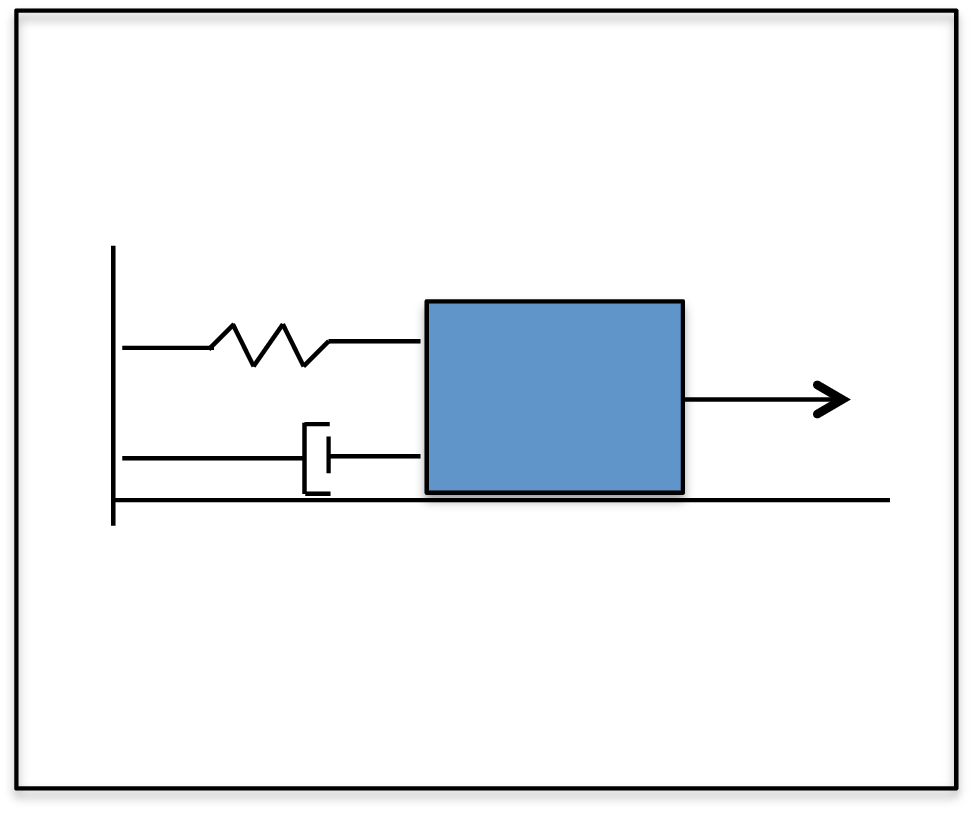
\includegraphics[width=0.1\textwidth]{6_design_studies/figures/hw_mass_thumbnail.pdf}}
		Homework \ref{hw:mass}.\ref{chap:PID-system-type}}  \label{hw:mass_system_type}
		\begin{description} \item[]
\item[(a)] Modify the state feedback solution developed in Homework~\ref{hw:vtol}.\ref{chap:state-feedback} to add an integrator with anti-windup to the altitude feedback loop and to the position feedback loop.
\item[(b)] Allow the plant parameters to vary up to 20\% and add a constant input disturbance of $0.1$~Newtons to the input of position dynamics simulating wind.  {\it Hint:  The best place to add the wind force is in the class that implements the dynamics.  For example, one possibility is to modify the $z$ dynamics as 

\texttt{zddot = (-(fr+fl)*sin(theta)+F\_wind)/(P.mc+2*P.mr)}.}

\item[(c)] Tune the integrator poles on both loops (and other gains if necessary) to get good tracking performance.  
\end{description}

%		\subsection*{Solution}
Python code used to design the observer based controller is shown below:
%\iftoggle{soln}{%
%  \lstinputlisting{simulink_e13/param.m}
%}{%
%  \lstinputlisting{./6_design_studies/_E_ballbeam/simulink/hw13/ballbeamParamHW13.m}
%}
\ifsolutionmanual
\lstinputlisting{./6_design_studies/_e_ballbeam/python/hw13/ballbeamParamHW13.py}
\else
\lstinputlisting{../../python/hw13/ballbeamParamHW13.py}
\fi


Python code for the observer based control  is shown below:
%\iftoggle{soln}{%
%  \lstinputlisting{simulink_e13/ballbeam_ctrl.m}
%}{%
%  \lstinputlisting{./6_design_studies/_E_ballbeam/simulink/hw13/ballbeam_ctrl.m}
%}
\ifsolutionmanual
\lstinputlisting{./6_design_studies/_e_ballbeam/python/hw13/ballBeamController.py}
\else
\lstinputlisting{../../python/hw13/ballBeamController.py}
\fi


See the wiki for the complete solution.


	\section*{
		\controlbookhyperref{hw:mass}{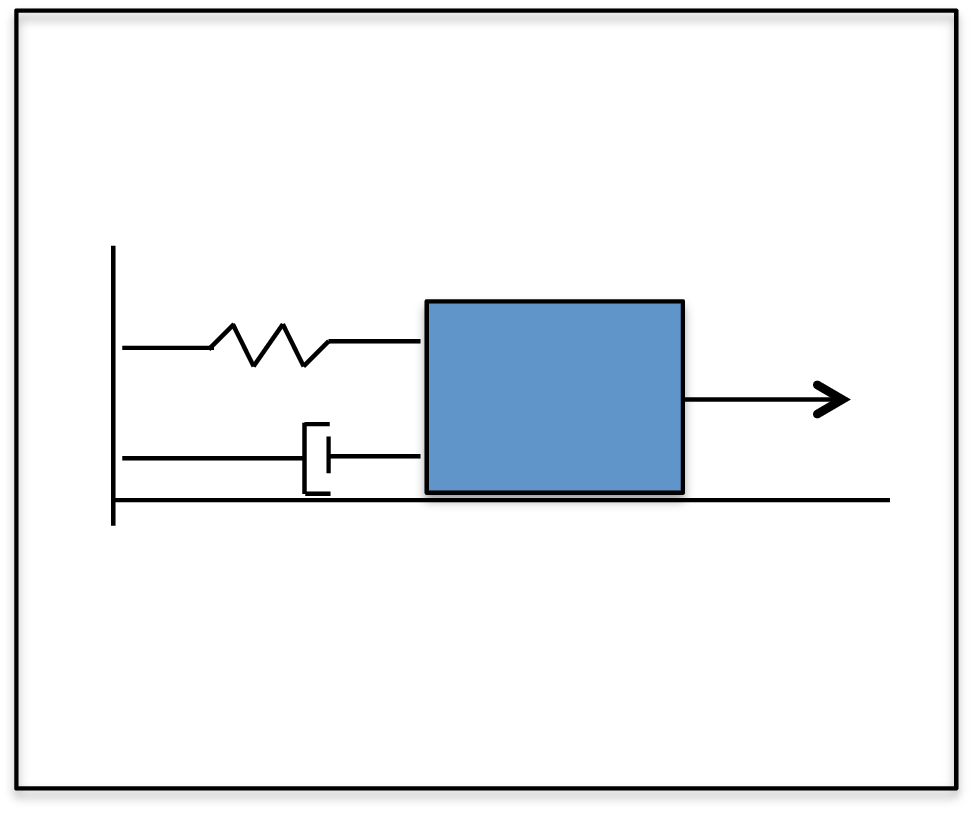
\includegraphics[width=0.1\textwidth]{6_design_studies/figures/hw_mass_thumbnail.pdf}}
		Homework \ref{hw:mass}.\ref{chap:PID-root-locus}}  \label{hw:mass_root_locus_PID}
		\begin{description} \item[]
\item[(a)] Modify the state feedback solution developed in Homework~\ref{hw:vtol}.\ref{chap:state-feedback} to add an integrator with anti-windup to the altitude feedback loop and to the position feedback loop.
\item[(b)] Allow the plant parameters to vary up to 20\% and add a constant input disturbance of $0.1$~Newtons to the input of position dynamics simulating wind.  {\it Hint:  The best place to add the wind force is in the class that implements the dynamics.  For example, one possibility is to modify the $z$ dynamics as 

\texttt{zddot = (-(fr+fl)*sin(theta)+F\_wind)/(P.mc+2*P.mr)}.}

\item[(c)] Tune the integrator poles on both loops (and other gains if necessary) to get good tracking performance.  
\end{description}

%		\subsection*{Solution}
Python code used to design the observer based controller is shown below:
%\iftoggle{soln}{%
%  \lstinputlisting{simulink_e13/param.m}
%}{%
%  \lstinputlisting{./6_design_studies/_E_ballbeam/simulink/hw13/ballbeamParamHW13.m}
%}
\ifsolutionmanual
\lstinputlisting{./6_design_studies/_e_ballbeam/python/hw13/ballbeamParamHW13.py}
\else
\lstinputlisting{../../python/hw13/ballbeamParamHW13.py}
\fi


Python code for the observer based control  is shown below:
%\iftoggle{soln}{%
%  \lstinputlisting{simulink_e13/ballbeam_ctrl.m}
%}{%
%  \lstinputlisting{./6_design_studies/_E_ballbeam/simulink/hw13/ballbeam_ctrl.m}
%}
\ifsolutionmanual
\lstinputlisting{./6_design_studies/_e_ballbeam/python/hw13/ballBeamController.py}
\else
\lstinputlisting{../../python/hw13/ballBeamController.py}
\fi


See the wiki for the complete solution.



%%%%%%%%%%%%%%% This is a root locus design problem. Please do not delete. Tim
%	\section*{
%		\controlbookhyperref{hw:mass}{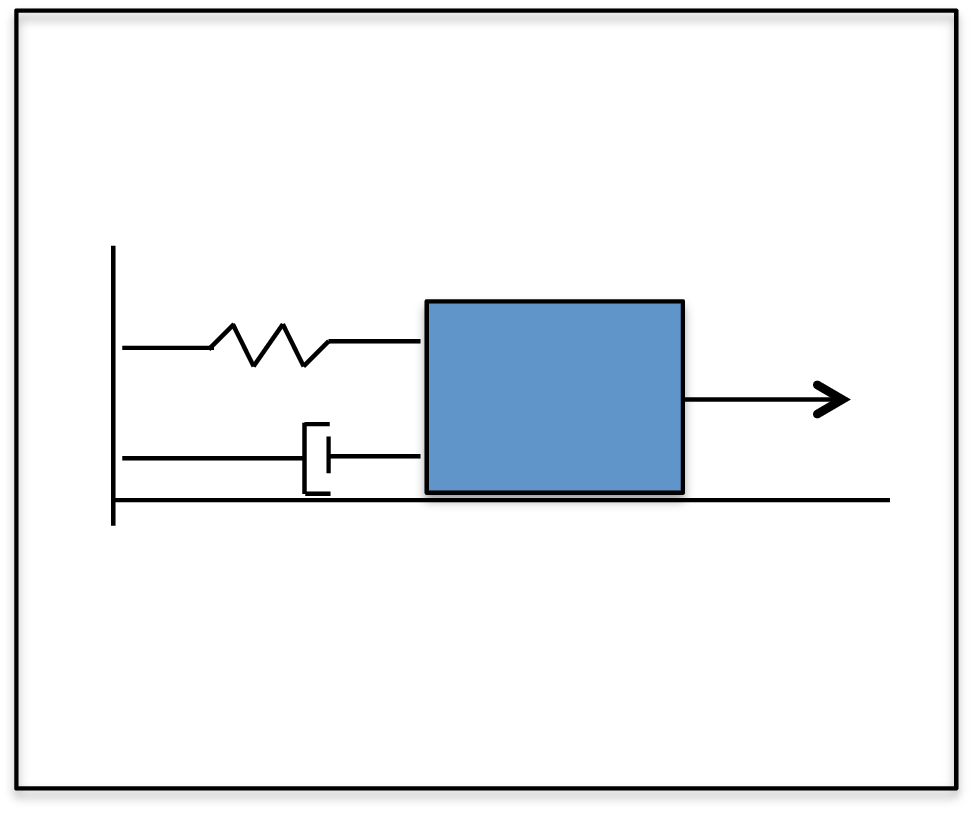
\includegraphics[width=0.1\textwidth]{6_design_studies/figures/hw_mass_thumbnail.pdf}}
%		Homework \ref{hw:mass}.\ref{chap:root-locus-design}}  \label{hw:mass_root_locus_design}
%		\begin{description} \item[]
\item[(a)] Modify the state feedback solution developed in Homework~\ref{hw:vtol}.\ref{chap:state-feedback} to add an integrator with anti-windup to the altitude feedback loop and to the position feedback loop.
\item[(b)] Allow the plant parameters to vary up to 20\% and add a constant input disturbance of $0.1$~Newtons to the input of position dynamics simulating wind.  {\it Hint:  The best place to add the wind force is in the class that implements the dynamics.  For example, one possibility is to modify the $z$ dynamics as 

\texttt{zddot = (-(fr+fl)*sin(theta)+F\_wind)/(P.mc+2*P.mr)}.}

\item[(c)] Tune the integrator poles on both loops (and other gains if necessary) to get good tracking performance.  
\end{description}

%%		\subsection*{Solution}
Python code used to design the observer based controller is shown below:
%\iftoggle{soln}{%
%  \lstinputlisting{simulink_e13/param.m}
%}{%
%  \lstinputlisting{./6_design_studies/_E_ballbeam/simulink/hw13/ballbeamParamHW13.m}
%}
\ifsolutionmanual
\lstinputlisting{./6_design_studies/_e_ballbeam/python/hw13/ballbeamParamHW13.py}
\else
\lstinputlisting{../../python/hw13/ballbeamParamHW13.py}
\fi


Python code for the observer based control  is shown below:
%\iftoggle{soln}{%
%  \lstinputlisting{simulink_e13/ballbeam_ctrl.m}
%}{%
%  \lstinputlisting{./6_design_studies/_E_ballbeam/simulink/hw13/ballbeam_ctrl.m}
%}
\ifsolutionmanual
\lstinputlisting{./6_design_studies/_e_ballbeam/python/hw13/ballBeamController.py}
\else
\lstinputlisting{../../python/hw13/ballBeamController.py}
\fi


See the wiki for the complete solution.



	\section*{
		\controlbookhyperref{hw:mass}{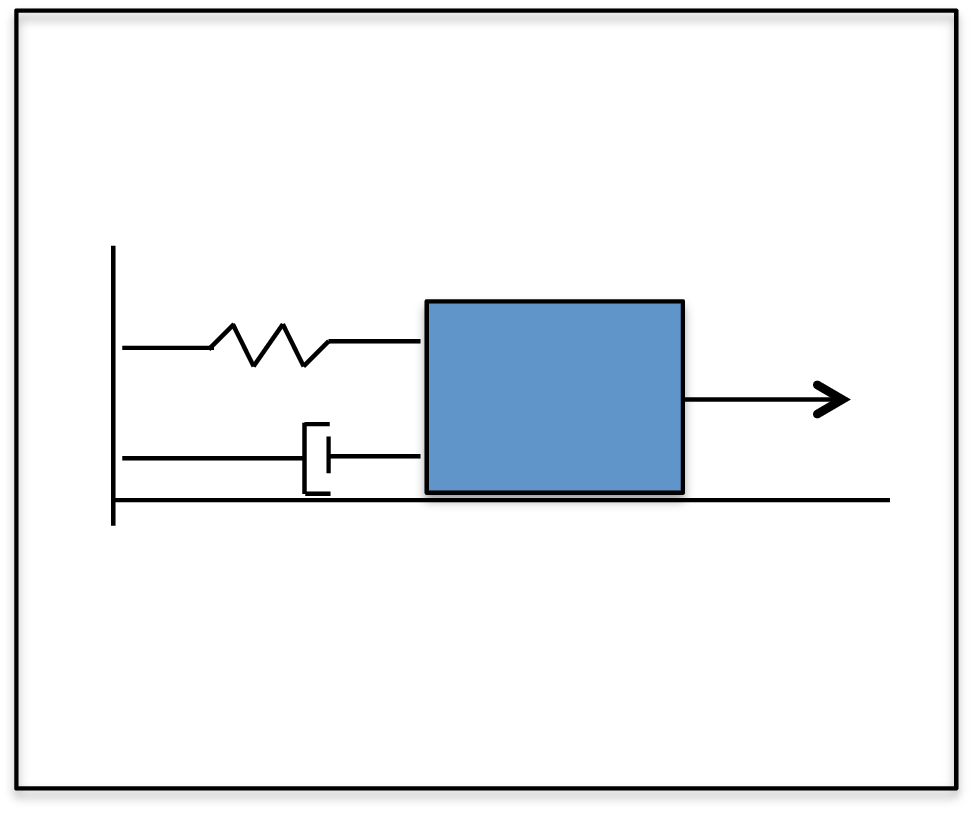
\includegraphics[width=0.1\textwidth]{6_design_studies/figures/hw_mass_thumbnail.pdf}}
		Homework \ref{hw:mass}.\ref{chap:PID-digital-implementation}}  \label{hw:mass_digital_PID}
		\begin{description} \item[]
\item[(a)] Modify the state feedback solution developed in Homework~\ref{hw:vtol}.\ref{chap:state-feedback} to add an integrator with anti-windup to the altitude feedback loop and to the position feedback loop.
\item[(b)] Allow the plant parameters to vary up to 20\% and add a constant input disturbance of $0.1$~Newtons to the input of position dynamics simulating wind.  {\it Hint:  The best place to add the wind force is in the class that implements the dynamics.  For example, one possibility is to modify the $z$ dynamics as 

\texttt{zddot = (-(fr+fl)*sin(theta)+F\_wind)/(P.mc+2*P.mr)}.}

\item[(c)] Tune the integrator poles on both loops (and other gains if necessary) to get good tracking performance.  
\end{description}

%		\subsection*{Solution}
Python code used to design the observer based controller is shown below:
%\iftoggle{soln}{%
%  \lstinputlisting{simulink_e13/param.m}
%}{%
%  \lstinputlisting{./6_design_studies/_E_ballbeam/simulink/hw13/ballbeamParamHW13.m}
%}
\ifsolutionmanual
\lstinputlisting{./6_design_studies/_e_ballbeam/python/hw13/ballbeamParamHW13.py}
\else
\lstinputlisting{../../python/hw13/ballbeamParamHW13.py}
\fi


Python code for the observer based control  is shown below:
%\iftoggle{soln}{%
%  \lstinputlisting{simulink_e13/ballbeam_ctrl.m}
%}{%
%  \lstinputlisting{./6_design_studies/_E_ballbeam/simulink/hw13/ballbeam_ctrl.m}
%}
\ifsolutionmanual
\lstinputlisting{./6_design_studies/_e_ballbeam/python/hw13/ballBeamController.py}
\else
\lstinputlisting{../../python/hw13/ballBeamController.py}
\fi


See the wiki for the complete solution.


	\section*{
		\controlbookhyperref{hw:mass}{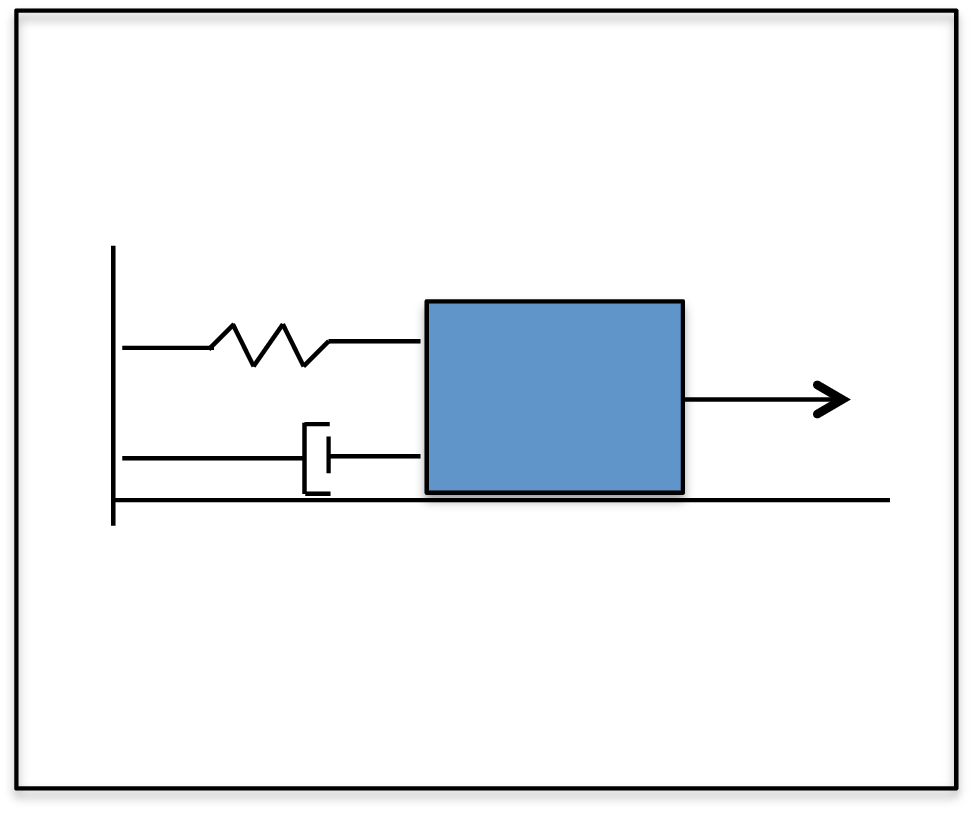
\includegraphics[width=0.1\textwidth]{6_design_studies/figures/hw_mass_thumbnail.pdf}}
		Homework \ref{hw:mass}.\ref{chap:state-feedback}}  \label{hw:mass_state_feedback}
		\begin{description} \item[]
\item[(a)] Modify the state feedback solution developed in Homework~\ref{hw:vtol}.\ref{chap:state-feedback} to add an integrator with anti-windup to the altitude feedback loop and to the position feedback loop.
\item[(b)] Allow the plant parameters to vary up to 20\% and add a constant input disturbance of $0.1$~Newtons to the input of position dynamics simulating wind.  {\it Hint:  The best place to add the wind force is in the class that implements the dynamics.  For example, one possibility is to modify the $z$ dynamics as 

\texttt{zddot = (-(fr+fl)*sin(theta)+F\_wind)/(P.mc+2*P.mr)}.}

\item[(c)] Tune the integrator poles on both loops (and other gains if necessary) to get good tracking performance.  
\end{description}

%		\subsection*{Solution}
Python code used to design the observer based controller is shown below:
%\iftoggle{soln}{%
%  \lstinputlisting{simulink_e13/param.m}
%}{%
%  \lstinputlisting{./6_design_studies/_E_ballbeam/simulink/hw13/ballbeamParamHW13.m}
%}
\ifsolutionmanual
\lstinputlisting{./6_design_studies/_e_ballbeam/python/hw13/ballbeamParamHW13.py}
\else
\lstinputlisting{../../python/hw13/ballbeamParamHW13.py}
\fi


Python code for the observer based control  is shown below:
%\iftoggle{soln}{%
%  \lstinputlisting{simulink_e13/ballbeam_ctrl.m}
%}{%
%  \lstinputlisting{./6_design_studies/_E_ballbeam/simulink/hw13/ballbeam_ctrl.m}
%}
\ifsolutionmanual
\lstinputlisting{./6_design_studies/_e_ballbeam/python/hw13/ballBeamController.py}
\else
\lstinputlisting{../../python/hw13/ballBeamController.py}
\fi


See the wiki for the complete solution.


	\section*{
		\controlbookhyperref{hw:mass}{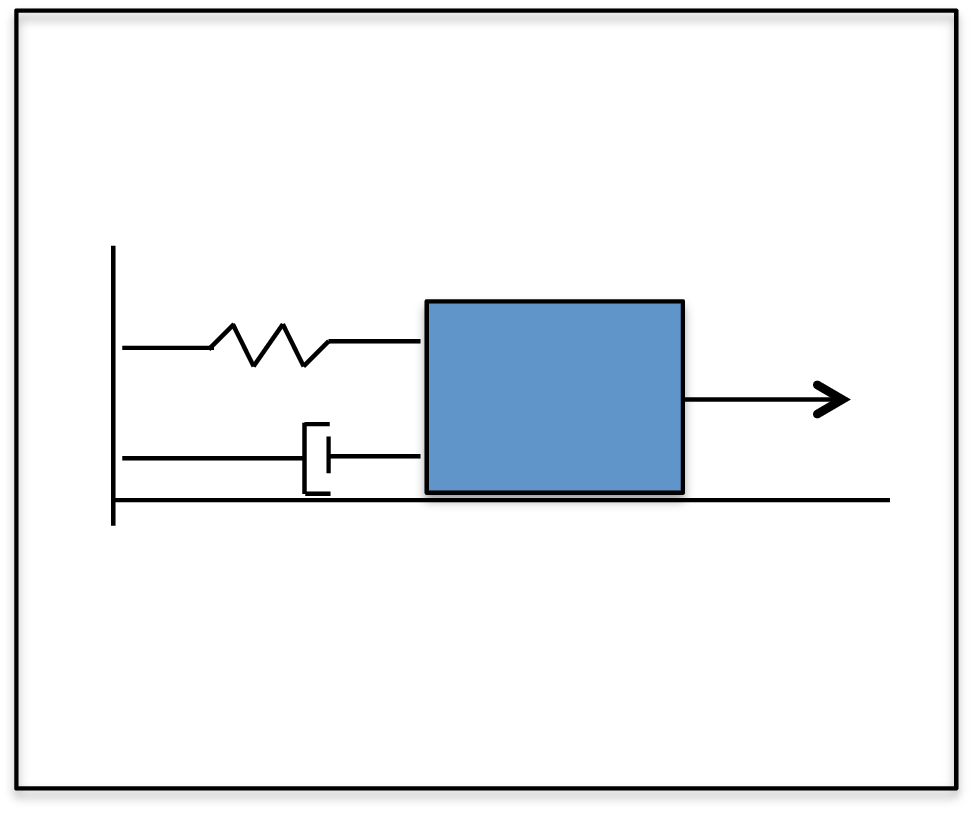
\includegraphics[width=0.1\textwidth]{6_design_studies/figures/hw_mass_thumbnail.pdf}}
		Homework \ref{hw:mass}.\ref{chap:state-feedback-integrator}}  \label{hw:mass_integrator_state_feedback}
		\begin{description} \item[]
\item[(a)] Modify the state feedback solution developed in Homework~\ref{hw:vtol}.\ref{chap:state-feedback} to add an integrator with anti-windup to the altitude feedback loop and to the position feedback loop.
\item[(b)] Allow the plant parameters to vary up to 20\% and add a constant input disturbance of $0.1$~Newtons to the input of position dynamics simulating wind.  {\it Hint:  The best place to add the wind force is in the class that implements the dynamics.  For example, one possibility is to modify the $z$ dynamics as 

\texttt{zddot = (-(fr+fl)*sin(theta)+F\_wind)/(P.mc+2*P.mr)}.}

\item[(c)] Tune the integrator poles on both loops (and other gains if necessary) to get good tracking performance.  
\end{description}

%		\subsection*{Solution}
Python code used to design the observer based controller is shown below:
%\iftoggle{soln}{%
%  \lstinputlisting{simulink_e13/param.m}
%}{%
%  \lstinputlisting{./6_design_studies/_E_ballbeam/simulink/hw13/ballbeamParamHW13.m}
%}
\ifsolutionmanual
\lstinputlisting{./6_design_studies/_e_ballbeam/python/hw13/ballbeamParamHW13.py}
\else
\lstinputlisting{../../python/hw13/ballbeamParamHW13.py}
\fi


Python code for the observer based control  is shown below:
%\iftoggle{soln}{%
%  \lstinputlisting{simulink_e13/ballbeam_ctrl.m}
%}{%
%  \lstinputlisting{./6_design_studies/_E_ballbeam/simulink/hw13/ballbeam_ctrl.m}
%}
\ifsolutionmanual
\lstinputlisting{./6_design_studies/_e_ballbeam/python/hw13/ballBeamController.py}
\else
\lstinputlisting{../../python/hw13/ballBeamController.py}
\fi


See the wiki for the complete solution.


	\section*{
		\controlbookhyperref{hw:mass}{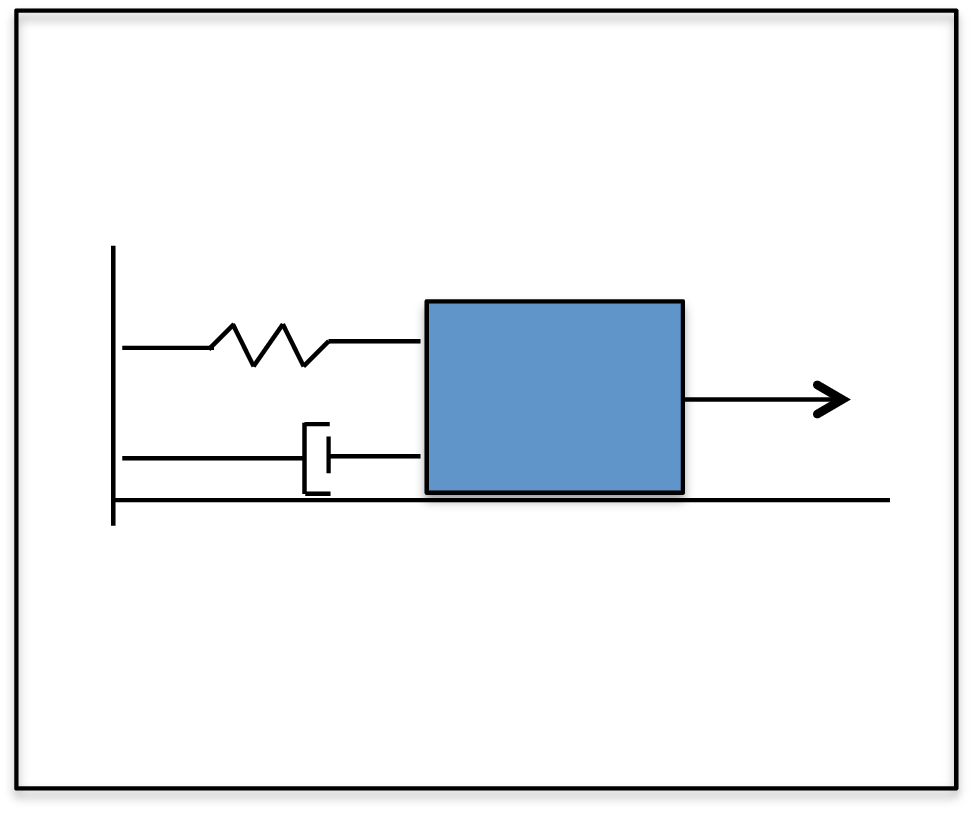
\includegraphics[width=0.1\textwidth]{6_design_studies/figures/hw_mass_thumbnail.pdf}}
		Homework \ref{hw:mass}.\ref{chap:observers}}  \label{hw:mass_observer}
		\begin{description} \item[]
\item[(a)] Modify the state feedback solution developed in Homework~\ref{hw:vtol}.\ref{chap:state-feedback} to add an integrator with anti-windup to the altitude feedback loop and to the position feedback loop.
\item[(b)] Allow the plant parameters to vary up to 20\% and add a constant input disturbance of $0.1$~Newtons to the input of position dynamics simulating wind.  {\it Hint:  The best place to add the wind force is in the class that implements the dynamics.  For example, one possibility is to modify the $z$ dynamics as 

\texttt{zddot = (-(fr+fl)*sin(theta)+F\_wind)/(P.mc+2*P.mr)}.}

\item[(c)] Tune the integrator poles on both loops (and other gains if necessary) to get good tracking performance.  
\end{description}

%		\subsection*{Solution}
Python code used to design the observer based controller is shown below:
%\iftoggle{soln}{%
%  \lstinputlisting{simulink_e13/param.m}
%}{%
%  \lstinputlisting{./6_design_studies/_E_ballbeam/simulink/hw13/ballbeamParamHW13.m}
%}
\ifsolutionmanual
\lstinputlisting{./6_design_studies/_e_ballbeam/python/hw13/ballbeamParamHW13.py}
\else
\lstinputlisting{../../python/hw13/ballbeamParamHW13.py}
\fi


Python code for the observer based control  is shown below:
%\iftoggle{soln}{%
%  \lstinputlisting{simulink_e13/ballbeam_ctrl.m}
%}{%
%  \lstinputlisting{./6_design_studies/_E_ballbeam/simulink/hw13/ballbeam_ctrl.m}
%}
\ifsolutionmanual
\lstinputlisting{./6_design_studies/_e_ballbeam/python/hw13/ballBeamController.py}
\else
\lstinputlisting{../../python/hw13/ballBeamController.py}
\fi


See the wiki for the complete solution.


	\section*{
		\controlbookhyperref{hw:mass}{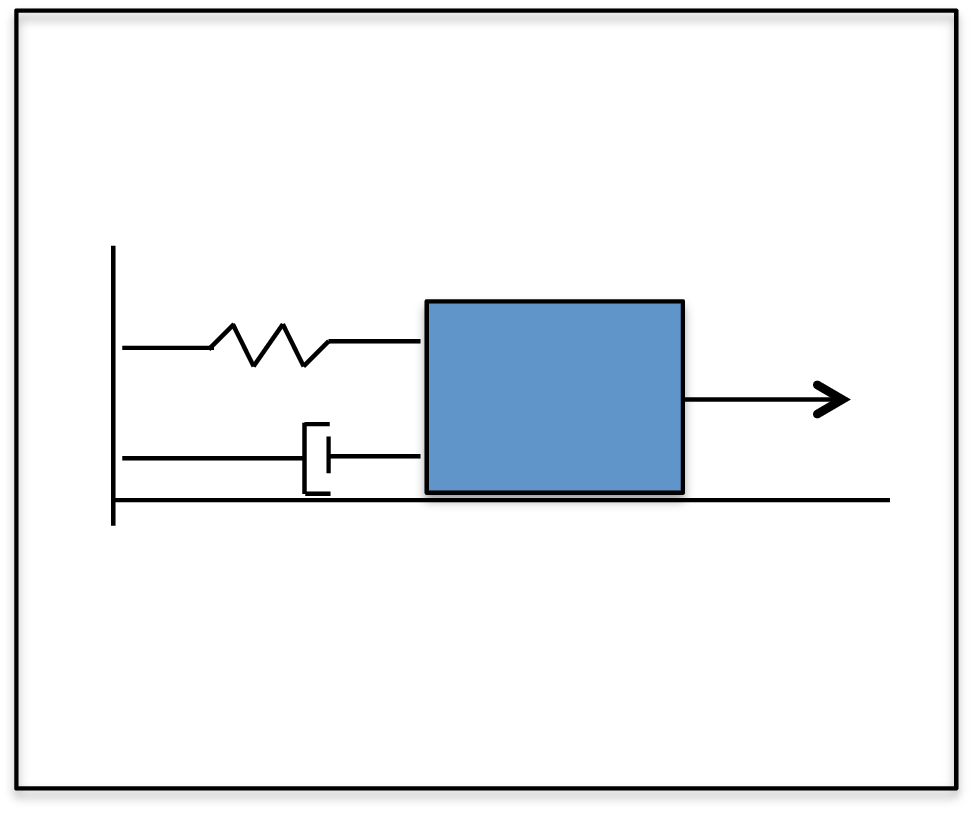
\includegraphics[width=0.1\textwidth]{6_design_studies/figures/hw_mass_thumbnail.pdf}}
		Homework \ref{hw:mass}.\ref{chap:disturbance_observers}}  \label{hw:mass_disturbance_observer}
		\begin{description} \item[]
\item[(a)] Modify the state feedback solution developed in Homework~\ref{hw:vtol}.\ref{chap:state-feedback} to add an integrator with anti-windup to the altitude feedback loop and to the position feedback loop.
\item[(b)] Allow the plant parameters to vary up to 20\% and add a constant input disturbance of $0.1$~Newtons to the input of position dynamics simulating wind.  {\it Hint:  The best place to add the wind force is in the class that implements the dynamics.  For example, one possibility is to modify the $z$ dynamics as 

\texttt{zddot = (-(fr+fl)*sin(theta)+F\_wind)/(P.mc+2*P.mr)}.}

\item[(c)] Tune the integrator poles on both loops (and other gains if necessary) to get good tracking performance.  
\end{description}

%		\subsection*{Solution}
Python code used to design the observer based controller is shown below:
%\iftoggle{soln}{%
%  \lstinputlisting{simulink_e13/param.m}
%}{%
%  \lstinputlisting{./6_design_studies/_E_ballbeam/simulink/hw13/ballbeamParamHW13.m}
%}
\ifsolutionmanual
\lstinputlisting{./6_design_studies/_e_ballbeam/python/hw13/ballbeamParamHW13.py}
\else
\lstinputlisting{../../python/hw13/ballbeamParamHW13.py}
\fi


Python code for the observer based control  is shown below:
%\iftoggle{soln}{%
%  \lstinputlisting{simulink_e13/ballbeam_ctrl.m}
%}{%
%  \lstinputlisting{./6_design_studies/_E_ballbeam/simulink/hw13/ballbeam_ctrl.m}
%}
\ifsolutionmanual
\lstinputlisting{./6_design_studies/_e_ballbeam/python/hw13/ballBeamController.py}
\else
\lstinputlisting{../../python/hw13/ballBeamController.py}
\fi


See the wiki for the complete solution.


	\section*{
		\controlbookhyperref{hw:mass}{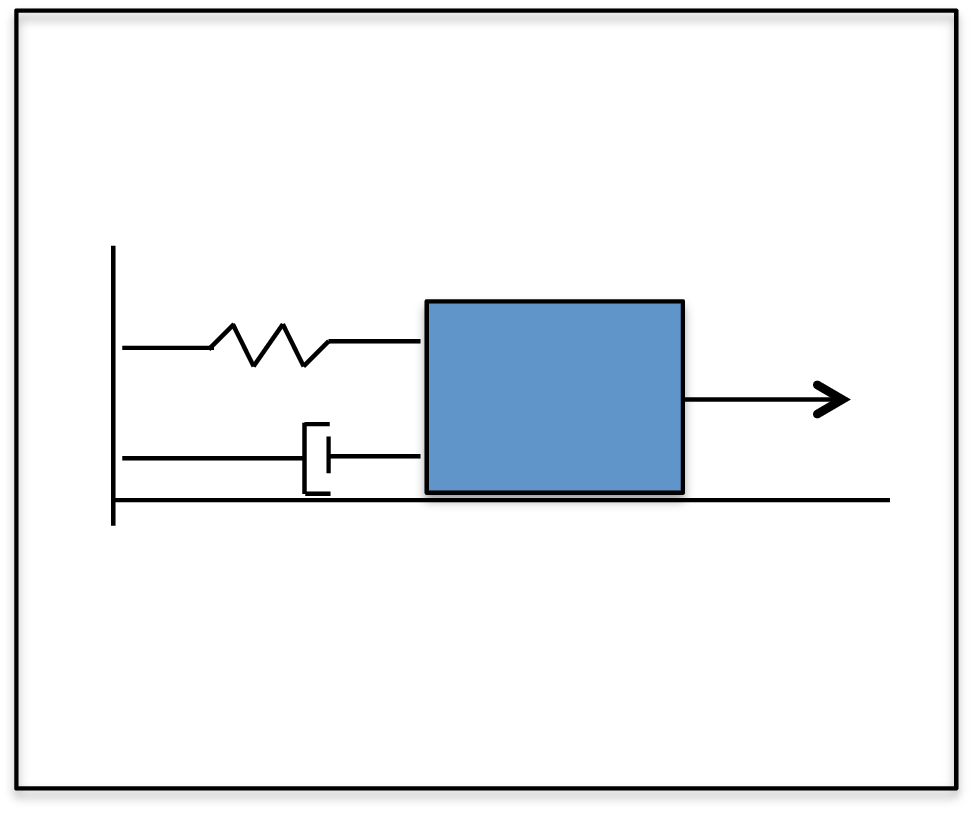
\includegraphics[width=0.1\textwidth]{6_design_studies/figures/hw_mass_thumbnail.pdf}}
		Homework \ref{hw:mass}.\ref{chap:bode_plots}}  \label{hw:mass_bode}
		\begin{description} \item[]
\item[(a)] Modify the state feedback solution developed in Homework~\ref{hw:vtol}.\ref{chap:state-feedback} to add an integrator with anti-windup to the altitude feedback loop and to the position feedback loop.
\item[(b)] Allow the plant parameters to vary up to 20\% and add a constant input disturbance of $0.1$~Newtons to the input of position dynamics simulating wind.  {\it Hint:  The best place to add the wind force is in the class that implements the dynamics.  For example, one possibility is to modify the $z$ dynamics as 

\texttt{zddot = (-(fr+fl)*sin(theta)+F\_wind)/(P.mc+2*P.mr)}.}

\item[(c)] Tune the integrator poles on both loops (and other gains if necessary) to get good tracking performance.  
\end{description}

%		\subsection*{Solution}
Python code used to design the observer based controller is shown below:
%\iftoggle{soln}{%
%  \lstinputlisting{simulink_e13/param.m}
%}{%
%  \lstinputlisting{./6_design_studies/_E_ballbeam/simulink/hw13/ballbeamParamHW13.m}
%}
\ifsolutionmanual
\lstinputlisting{./6_design_studies/_e_ballbeam/python/hw13/ballbeamParamHW13.py}
\else
\lstinputlisting{../../python/hw13/ballbeamParamHW13.py}
\fi


Python code for the observer based control  is shown below:
%\iftoggle{soln}{%
%  \lstinputlisting{simulink_e13/ballbeam_ctrl.m}
%}{%
%  \lstinputlisting{./6_design_studies/_E_ballbeam/simulink/hw13/ballbeam_ctrl.m}
%}
\ifsolutionmanual
\lstinputlisting{./6_design_studies/_e_ballbeam/python/hw13/ballBeamController.py}
\else
\lstinputlisting{../../python/hw13/ballBeamController.py}
\fi


See the wiki for the complete solution.


	\section*{
		\controlbookhyperref{hw:mass}{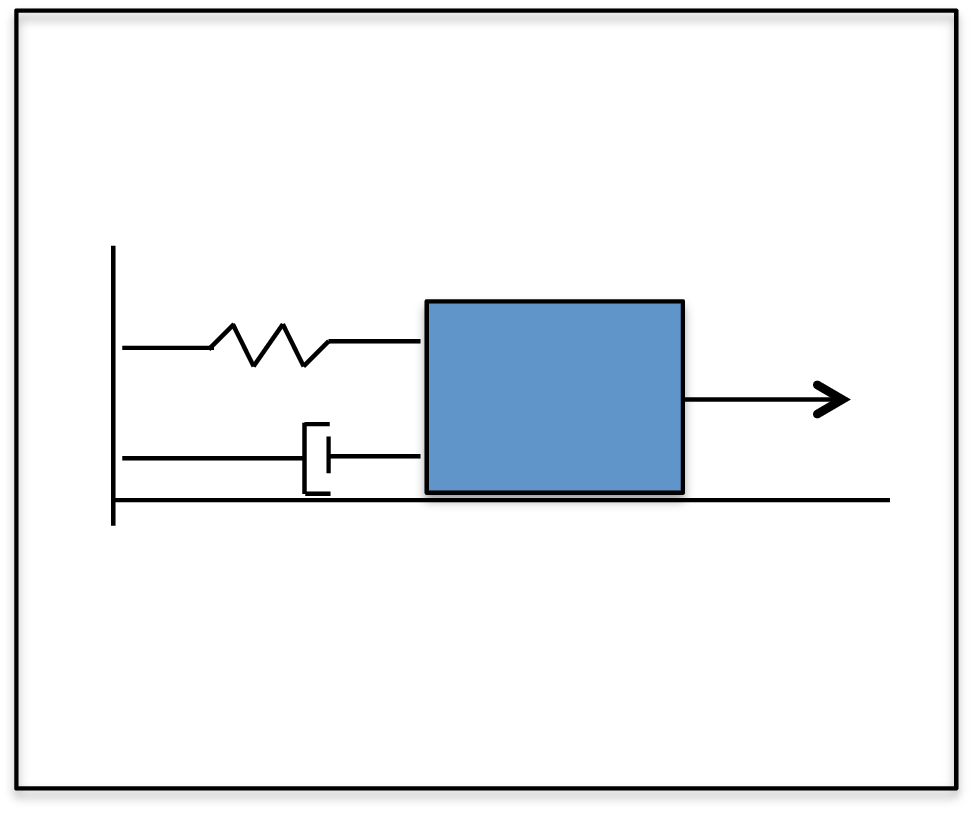
\includegraphics[width=0.1\textwidth]{6_design_studies/figures/hw_mass_thumbnail.pdf}}
		Homework \ref{hw:mass}.\ref{chap:tracking_disturbance_noise}}  \label{hw:mass_loopgain}
		\begin{description} \item[]
\item[(a)] Modify the state feedback solution developed in Homework~\ref{hw:vtol}.\ref{chap:state-feedback} to add an integrator with anti-windup to the altitude feedback loop and to the position feedback loop.
\item[(b)] Allow the plant parameters to vary up to 20\% and add a constant input disturbance of $0.1$~Newtons to the input of position dynamics simulating wind.  {\it Hint:  The best place to add the wind force is in the class that implements the dynamics.  For example, one possibility is to modify the $z$ dynamics as 

\texttt{zddot = (-(fr+fl)*sin(theta)+F\_wind)/(P.mc+2*P.mr)}.}

\item[(c)] Tune the integrator poles on both loops (and other gains if necessary) to get good tracking performance.  
\end{description}

%		\subsection*{Solution}
Python code used to design the observer based controller is shown below:
%\iftoggle{soln}{%
%  \lstinputlisting{simulink_e13/param.m}
%}{%
%  \lstinputlisting{./6_design_studies/_E_ballbeam/simulink/hw13/ballbeamParamHW13.m}
%}
\ifsolutionmanual
\lstinputlisting{./6_design_studies/_e_ballbeam/python/hw13/ballbeamParamHW13.py}
\else
\lstinputlisting{../../python/hw13/ballbeamParamHW13.py}
\fi


Python code for the observer based control  is shown below:
%\iftoggle{soln}{%
%  \lstinputlisting{simulink_e13/ballbeam_ctrl.m}
%}{%
%  \lstinputlisting{./6_design_studies/_E_ballbeam/simulink/hw13/ballbeam_ctrl.m}
%}
\ifsolutionmanual
\lstinputlisting{./6_design_studies/_e_ballbeam/python/hw13/ballBeamController.py}
\else
\lstinputlisting{../../python/hw13/ballBeamController.py}
\fi


See the wiki for the complete solution.


	\section*{
		\controlbookhyperref{hw:mass}{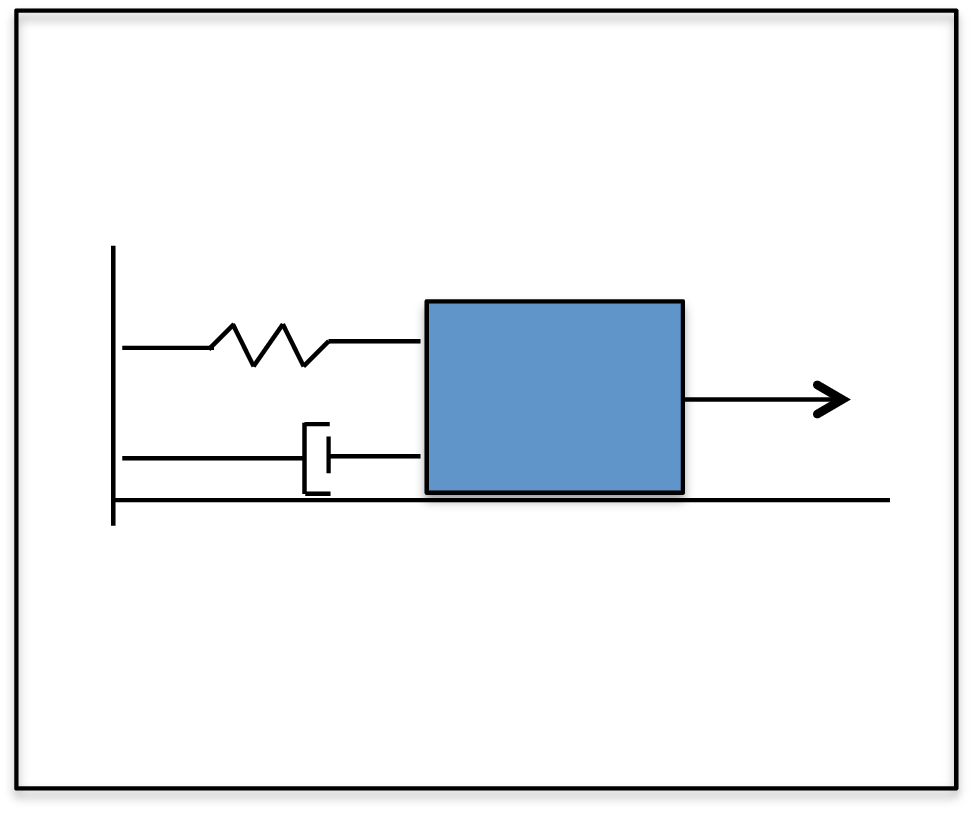
\includegraphics[width=0.1\textwidth]{6_design_studies/figures/hw_mass_thumbnail.pdf}}
		Homework \ref{hw:mass}.\ref{chap:margins}}  \label{hw:mass_margins}
		\begin{description} \item[]
\item[(a)] Modify the state feedback solution developed in Homework~\ref{hw:vtol}.\ref{chap:state-feedback} to add an integrator with anti-windup to the altitude feedback loop and to the position feedback loop.
\item[(b)] Allow the plant parameters to vary up to 20\% and add a constant input disturbance of $0.1$~Newtons to the input of position dynamics simulating wind.  {\it Hint:  The best place to add the wind force is in the class that implements the dynamics.  For example, one possibility is to modify the $z$ dynamics as 

\texttt{zddot = (-(fr+fl)*sin(theta)+F\_wind)/(P.mc+2*P.mr)}.}

\item[(c)] Tune the integrator poles on both loops (and other gains if necessary) to get good tracking performance.  
\end{description}

%		\subsection*{Solution}
Python code used to design the observer based controller is shown below:
%\iftoggle{soln}{%
%  \lstinputlisting{simulink_e13/param.m}
%}{%
%  \lstinputlisting{./6_design_studies/_E_ballbeam/simulink/hw13/ballbeamParamHW13.m}
%}
\ifsolutionmanual
\lstinputlisting{./6_design_studies/_e_ballbeam/python/hw13/ballbeamParamHW13.py}
\else
\lstinputlisting{../../python/hw13/ballbeamParamHW13.py}
\fi


Python code for the observer based control  is shown below:
%\iftoggle{soln}{%
%  \lstinputlisting{simulink_e13/ballbeam_ctrl.m}
%}{%
%  \lstinputlisting{./6_design_studies/_E_ballbeam/simulink/hw13/ballbeam_ctrl.m}
%}
\ifsolutionmanual
\lstinputlisting{./6_design_studies/_e_ballbeam/python/hw13/ballBeamController.py}
\else
\lstinputlisting{../../python/hw13/ballBeamController.py}
\fi


See the wiki for the complete solution.


	\section*{
		\controlbookhyperref{hw:mass}{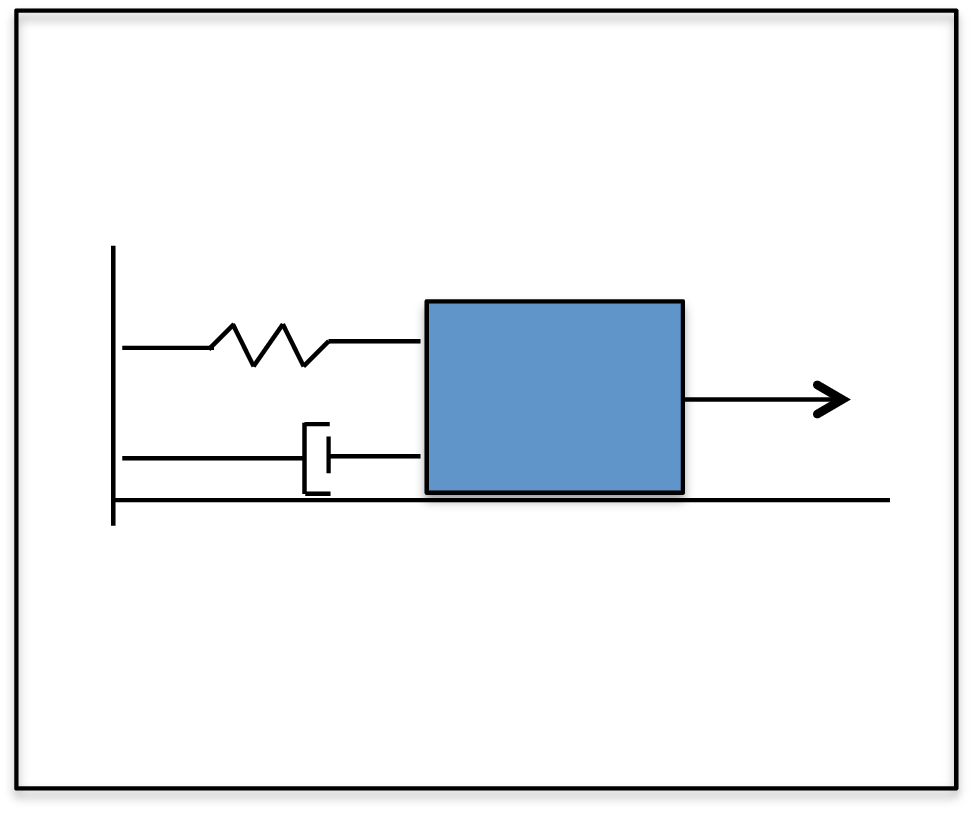
\includegraphics[width=0.1\textwidth]{6_design_studies/figures/hw_mass_thumbnail.pdf}}
		Homework \ref{hw:mass}.\ref{chap:loopshaping_design}}  \label{hw:mass_loopshaping}
		\begin{description} \item[]
\item[(a)] Modify the state feedback solution developed in Homework~\ref{hw:vtol}.\ref{chap:state-feedback} to add an integrator with anti-windup to the altitude feedback loop and to the position feedback loop.
\item[(b)] Allow the plant parameters to vary up to 20\% and add a constant input disturbance of $0.1$~Newtons to the input of position dynamics simulating wind.  {\it Hint:  The best place to add the wind force is in the class that implements the dynamics.  For example, one possibility is to modify the $z$ dynamics as 

\texttt{zddot = (-(fr+fl)*sin(theta)+F\_wind)/(P.mc+2*P.mr)}.}

\item[(c)] Tune the integrator poles on both loops (and other gains if necessary) to get good tracking performance.  
\end{description}

%		\subsection*{Solution}
Python code used to design the observer based controller is shown below:
%\iftoggle{soln}{%
%  \lstinputlisting{simulink_e13/param.m}
%}{%
%  \lstinputlisting{./6_design_studies/_E_ballbeam/simulink/hw13/ballbeamParamHW13.m}
%}
\ifsolutionmanual
\lstinputlisting{./6_design_studies/_e_ballbeam/python/hw13/ballbeamParamHW13.py}
\else
\lstinputlisting{../../python/hw13/ballbeamParamHW13.py}
\fi


Python code for the observer based control  is shown below:
%\iftoggle{soln}{%
%  \lstinputlisting{simulink_e13/ballbeam_ctrl.m}
%}{%
%  \lstinputlisting{./6_design_studies/_E_ballbeam/simulink/hw13/ballbeam_ctrl.m}
%}
\ifsolutionmanual
\lstinputlisting{./6_design_studies/_e_ballbeam/python/hw13/ballBeamController.py}
\else
\lstinputlisting{../../python/hw13/ballBeamController.py}
\fi


See the wiki for the complete solution.





